\chapter{Der Allgemeine Workflow in TensorFlow}

Zu Beginn dieses Kapitels wird die Methodik der Aufteilung der Datensätze in Trainings-, Validierungs- und Testdaten erläutert, welches für die Beurteilung der Ergebnisse eines Modells unerlässlich ist. Anschließend erfolgt eine Einführung in das Visualisierungstool TensorBoard, mit dessen Hilfe sich die hier vorgestellten und noch weitere Vorgänge anschaulich abbilden lassen. Am Schluss werden noch die einzelnen Graphelemente näher betrachtet, wodurch sich umfangreiche Graphabbildungen erzeugen lassen. 
%\section{Die Tooling Pipeline}


\section{Vorgehensweise beim Trainingsprozess}


Eines der entscheidenden Kriterien über die Qualität des Modells ist die Prognose der Zielgröße auf zuvor ungesehenen Daten. Die Genauigkeit auf den Daten, mit denen das Modell trainiert wurde, geben keine grundlegende Aussage über die zu erwartende Genauigkeit auf zukünftige Daten. Deshalb ist es essentiell wichtig ungenutzte Testdaten zur Beurteilung mit einzubeziehen. Häufig müssen Entscheidungen über Metaparameter wie Neuronenanzahl, Stärke der Regularisierung, Art des Kernels getroffen werden. Daher unterteilt man die Datensätze in Trainings-, Validierungs- und Testdaten \cite{hoffmann2014proceedings}.
\vspace{10pt}

\begin{itemize} 
\item \textbf{Training} \vspace{5pt}

Trainingsdaten bilden die Grundlage für das überwachte Lernen. Hierbei werden durch eine Reihe von Beispielen Parameter wie die Gewichte der Verbindungen zwischen den Neuronen angepasst. Häufig besteht der Trainingsdatensatz aus Paaren von Eingangsvektoren und der dazugehörigen Antwortvektoren. \vspace{10pt}

\item \textbf{Validierung} \vspace{5pt}

Validierungsdaten dienen der Festlegung der optimalen Struktur des Modells, insbesondere zur Einstellung der optimalen Parameter des Lernalgorithmus wie die Lernrate oder die Anzahl der Trainingsepochen. Validierungsdatensätze werden auch für die Regularisierung von  \dq early stopping\grqq{} und bei der Zunahme des Fehlers im Validierungsdatensatz, da dies ein Zeichen für  \dq overfitting\grqq{} ist, angewandt. \vspace{10pt}

\item \textbf{Testen} \vspace{5pt}

Testdaten werden verwendet, um eine Bewertung eines endgültigen Modells zu ermöglichen, welche auf ungesehene Daten angewandt wurde.

\end{itemize}\vspace{10pt}


\textbf{Cross-Validation} \vspace{10pt}

Die Unterteilung des Datensatzes in einen festen Trainingssatz und einen festen Testsatz kann problematisch sein, wenn der Testsatz zu klein ist. Dies impliziert statistische Unsicherheit im Bereich des geschätzten Testfehlers. Abhilfe schafft die k-fache Kreuzvalidierung (Cross-Validation), welche die Daten in k disjunkte Teilmengen unterteilt, auf denen k Tests durchgeführt werden, wobei jeweils k-1 Teilmengen für das Training und die verbliebene Teilmenge zum Testen verwendet wird \cite{hoffmann2014proceedings}.

%https://books.google.de/books?id=93djocO3yVgC&hl=de&source=gbs_navlinks_s
%Proceedings. 22. Workshop Computational Intelligence, Dortmund, 6. - 7. Dezember 2012

\section{Die Visualisierung mit TensorBoard}

TensorBoard ist eine in TensorFlow enthaltene Webanwendung zur Visualisierung der Abläufe in einem neuronalen Netz. TensorBoard stellt eine Vielzahl an graphischen Elementen zur Verfügung, welche dem Entwickler vorallem das Debuggen oder die Optimierung eines erstellten Modells erleichtern. Ebenso können damit insbesondere komplexe Datenstrukturen zum besseren Verständnis anschaulich visualisiert werden. 

Bevor mit TensorBoard gearbeitet werden kann, muss nachfolgender Befehl in die Kommandozeile eingegeben werden:
\\

\begin{minipage}{\linewidth}
\begin{lstlisting}[language=bash, label={lst:tensorboard}]
C:\> tensorboard  --logdir=path/to/log_directory

\end{lstlisting}
\end{minipage}

\vspace{0.2cm}
wobei vorher im spezifizierten Log Ordner die gewünschten Event Daten mit der Klasse
\\

\begin{minipage}{\linewidth}
\begin{lstlisting}[language=Python, label={lst:FileWriter}]
tf.summary.FileWriter('path/to/log_directory')

\end{lstlisting}
\end{minipage}
\vspace{0.2cm}

abgespeichert werden müssen. Nachdem TensorBoard gestart wurde, navigiert man mit dem Browser zu folgender Seite:
\\

\begin{minipage}{\linewidth}
\begin{lstlisting}[language=Python, label={lst:FileWriter}]
http://localhost:6006

\end{lstlisting}
\end{minipage}
\vspace{0.2cm}

Falls keine Fehlermeldungen aufgetreten sind, sollte folgender Bildschirminhalt Abbildung \ref{fig:tensorboard_start} angezeigt werden. Um die Visualisierungen in den einzelnen Reiter zu erhalten, müssen diese vorher im Programm mit speziellen TensorFlow Klassen abgespeichert werden. In dem nachfolgenden Kapitel werden die einzelnen Reiter und der dazugehörigen Klasse vorgestellt. 
\\[1ex]

\begin{figure}[h!]
	\centering
	%\vspace{-35pt}
	%\hspace{-1.0cm} 
	 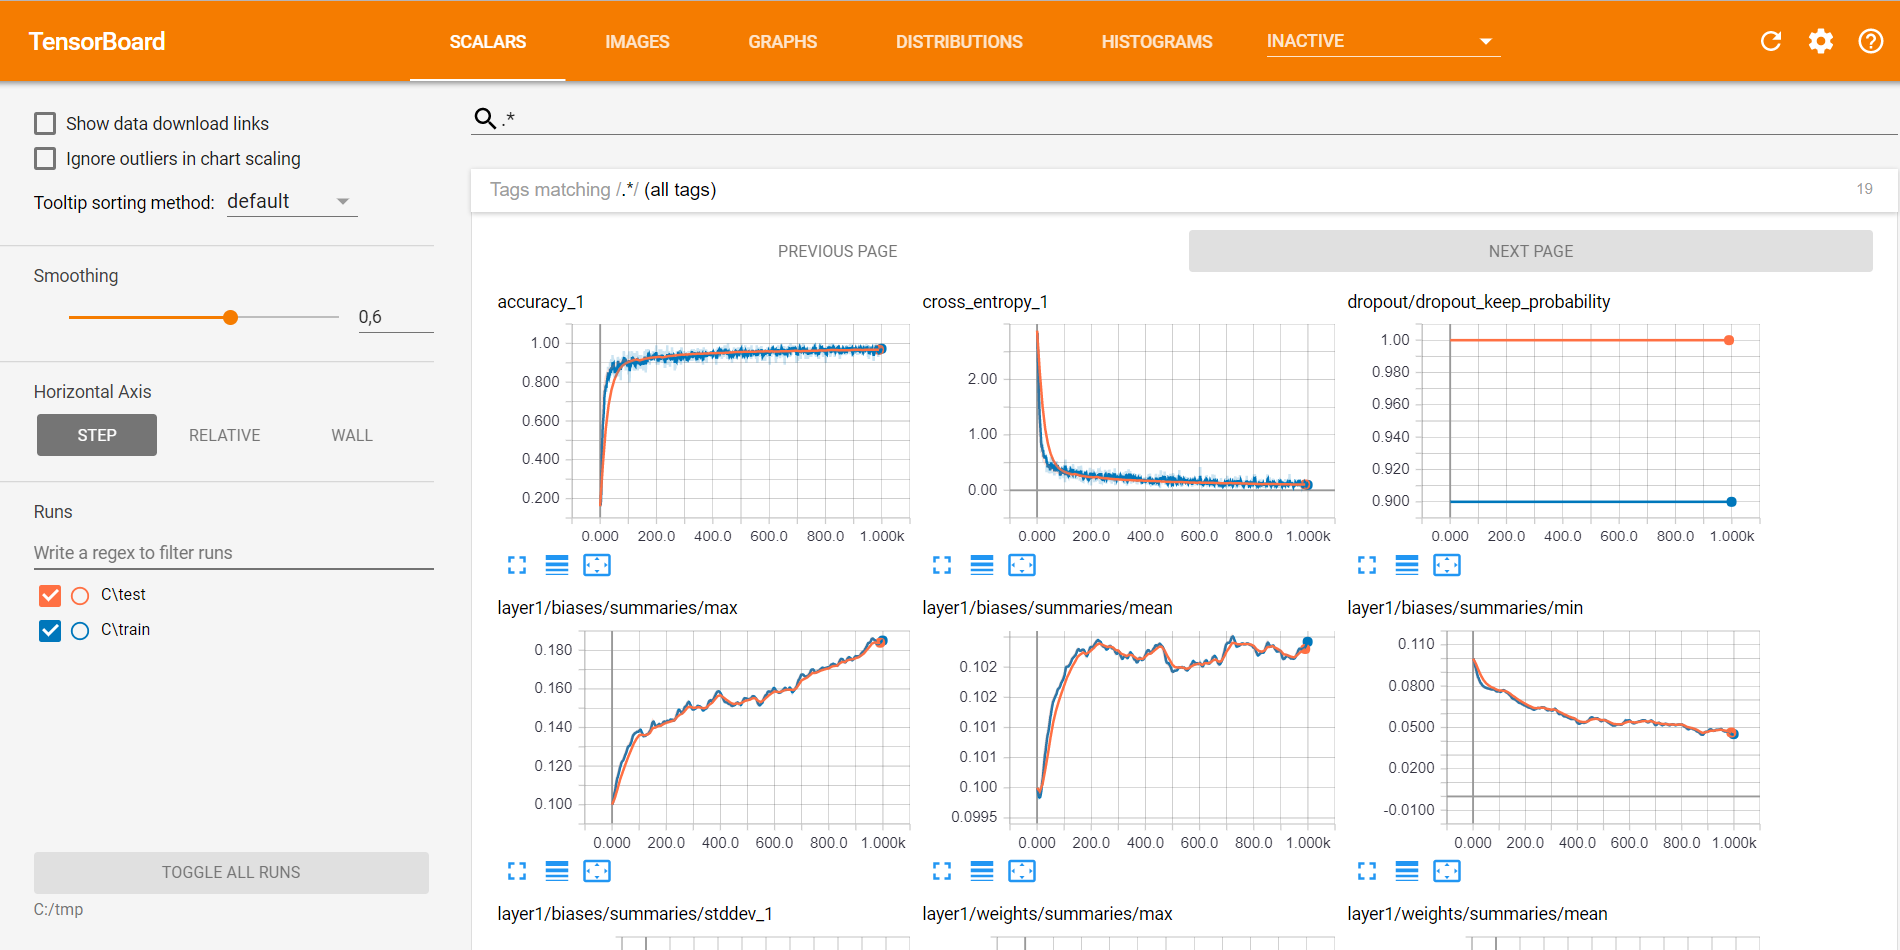
\includegraphics[width=1\textwidth]{images/Kapitel_3/TensorBoard_start.png}\\
	\vspace{10pt} 
	\caption[Die Startseite von TensorBoard]{Die Startseite von TensorBoard}
	\label{fig:tensorboard_start}
\end{figure}





\section{Die einzelnen Visualisierungsmöglichkeiten im Detail}

\subsection{Skalare}
%\textbf{\textit{Skalare}} 
\vspace{10pt}
Unter dem Reiter Skalare, welche mit der Klasse
\\

\begin{minipage}{\linewidth}
\begin{lstlisting} [label={lst:scalar}]
tf.summary.scalar(name, tensor, collections=None, family=None)
\end{lstlisting}
\end{minipage}

\vspace{0.2cm}

abgespeichert werden, können verschiedenste Statistiken während eines Trainingsprozesses visualisiert werden. Dies könnten zum Beispiel die Genauigkeit oder Cross-Entropie sein, welche in Abbildung \ref{fig:skalare} dargestellt sind. Hierbei wird die Genauigkeit über den einzelnen Trainingsschritten aufgetragen. Wählt man mit der Maus einen bestimmten Datenpunkt aus, so werden zahlreiche weitere Informationen angezeigt. Ebenso ist hierbei ersichtlich, dass auch Trainings- und Testdaten gleichzeitig angezeigt und miteinander verglichen werden können \cite{tensorboard.2017}.

\begin{figure}[h!]
	\centering
	%\vspace{-35pt}
	%\hspace{-1.0cm} 
	 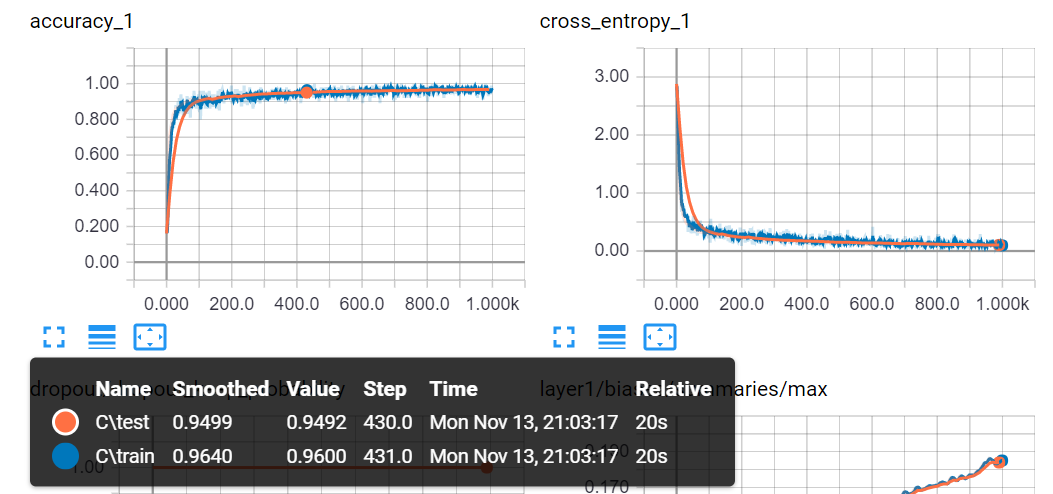
\includegraphics[width=0.8\textwidth]{images/Kapitel_3/skalars.png}\\
	\vspace{10pt} 
	\caption[Visualisierung der 'Accuracy' und 'Cross\_entropy' über die einzelnen Trainingsschritte]{Visualisierung der 'Accuracy' und 'Cross\_entropy' über die einzelnen Trainingschritte}
	\label{fig:skalare}
\end{figure}





\subsection{Bilder}
%\textbf{\textit{Bilder}}
%\vspace{30pt}

Innerhalb des Reiters Bilder, welche mit der Klasse
\\

\begin{minipage}{\linewidth}
\begin{lstlisting} [label={lst:scalar}]
tf.summary.image(name, tensor, max_outputs=3, collections=None, family=None)
\end{lstlisting}
\end{minipage}


\begin{figure}[htb!]
	\centering
     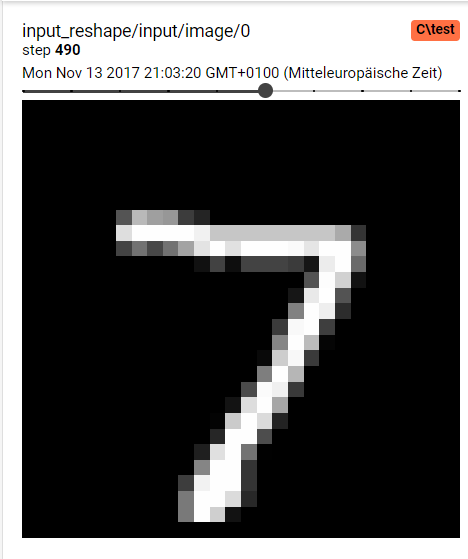
\includegraphics[width=6cm]{images/Kapitel_3/images.png}
	\vspace{10pt} 
	\caption{Bild des Testschrittes 490}
	\label{fig:DBvsTF}
\end{figure}

abgespeichert werden, können zur genaueren Analyse die Test- und Trainingsbilder eingesehen werden. 
Über den Bildern ist eine Scrollbar vorhanden mit dieser können einzelne Test- und Trainingsschritte ausgewählt werden, wodurch genau ersichtlich wird, welches Bild zum aktuellen Durchlauf gehört \cite{tensorboard.2017}.
\vspace{50pt}
\newpage


\begin{figure}[t]
\begin{minipage}[t]{0.475\textwidth}
\centering
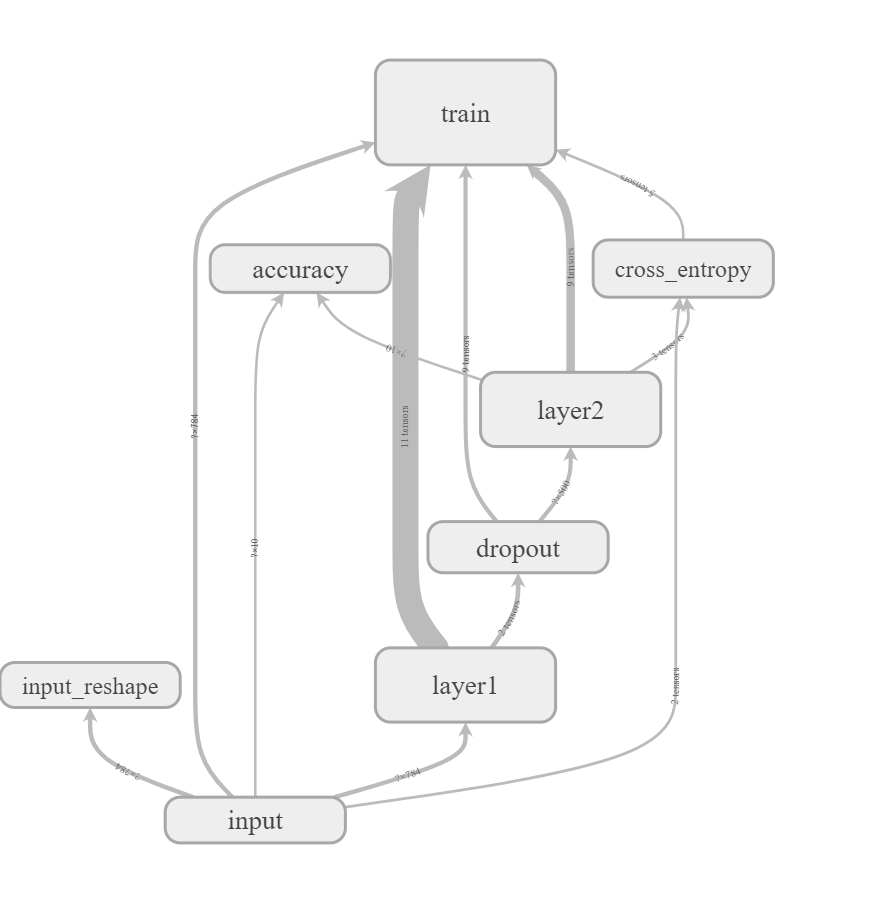
\includegraphics[width=0.9\textwidth]{images/Kapitel_3/graph.png}
\caption{TensorFlow Graph mit definierten Name scopes}
\label{fig:TensorFlow_Graph}
\end{minipage}
\hfill
\begin{minipage}[t]{0.475\textwidth}
\centering
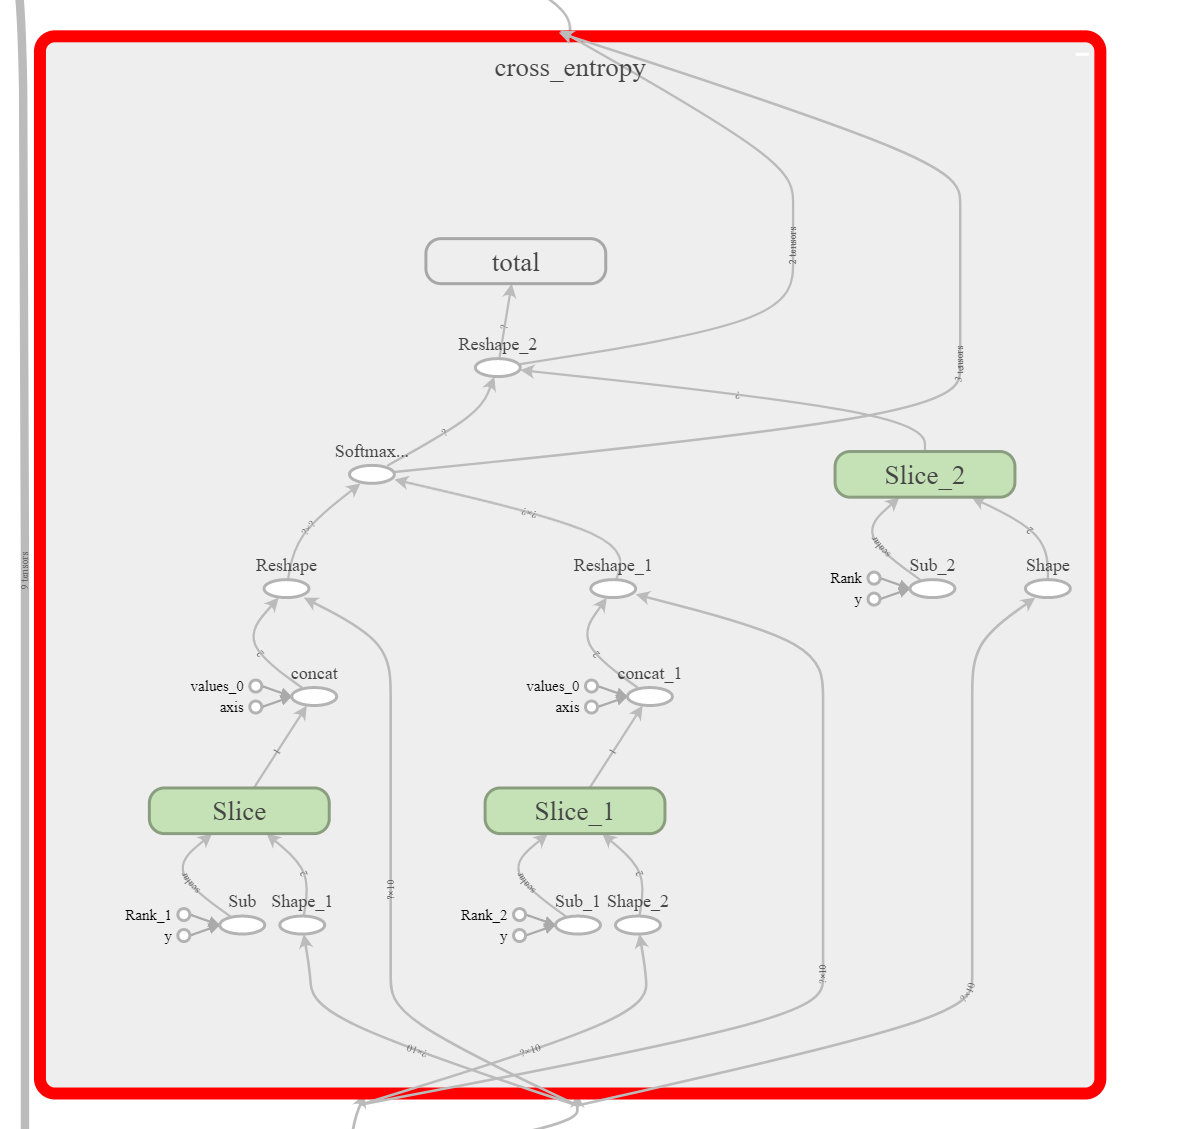
\includegraphics[width=0.9\textwidth]{images/Kapitel_3/graph1.png}
\caption{Name scope 'cross\_entropy' unterteilt in weiteren Operationen}
\label{fig:name_scope_cross_entropy}
\end{minipage}
\end{figure}



\subsection{Graphen} \label{sub:tb-graph}
%\textbf{\textit{Graphen}}
\vspace{10pt}
Unter dem Reiter Graphen befindet sich das komplette TensorFlow Model als Graph,  wie in Abbildung \ref{fig:TensorFlow_Graph} zu sehen ist. Nur wenn im erstellten Programm vorher Name scopes definiert wurden, zeigt TensorBoard den Graphen an. Um Graphen in Tensorboard zu erhalten, müssen die gewünschten Operationen als Name scope erstellt werden. Mit nachfolgendem Befehl in Zeile 1 erhält man einen \textit{cross\_entropy} Name scope: 
\\

\begin{minipage}{\linewidth}
\begin{lstlisting} [label={lst:scalar}]
with tf.name_scope('cross_entropy'):
  diff = tf.nn.softmax_cross_entropy_with_logits(targets=y_, logits=y)
  with tf.name_scope('total'):
    cross_entropy = tf.reduce_mean(diff)
tf.summary.scalar('cross_entropy', cross_entropy)
\end{lstlisting}
\end{minipage}
\vspace{0.2cm}

Der Name scope \textit{cross\_entropy} in Abbildung \ref{fig:name_scope_cross_entropy} kann natürlich wiederum in mehrere Untergruppierungen aufgeteilt werden. So erhält man eine übersichtliche Visualisierung komplexer TensorFlow Modelle \cite{tensorboard.2017}.






\subsection{Histogramme}
%\textbf{\textit{Histogramme}}
\vspace{10pt}
Unter dem Reiter Histogramme, welche mit der Klasse
\\

\begin{minipage}{\linewidth}
\begin{lstlisting} [label={lst:scalar}]
tf.summary.histogram(name, values, collections=None, familiy=None)
\end{lstlisting}
\end{minipage}
\vspace{0.2cm}


abgespeichert werden, wird die statistische Verteilung eines Tensors über der Zeit dargestellt. Im Histogramm sind zeitliche \dq Slices\grqq{} der Daten visualisiert, wobei jeder einzelne Slice ein Histogramm des Tensors in einem einzelnen Schritt darstellt. In Abbildung \ref{fig:histogram} ist ein einzelner Slice schwarz markiert \cite{tensorboard.2017}.

\vspace{0.6cm}
\begin{figure}[h!]
	\centering
	%\vspace{-35pt}
	%\hspace{-1.0cm} 
	 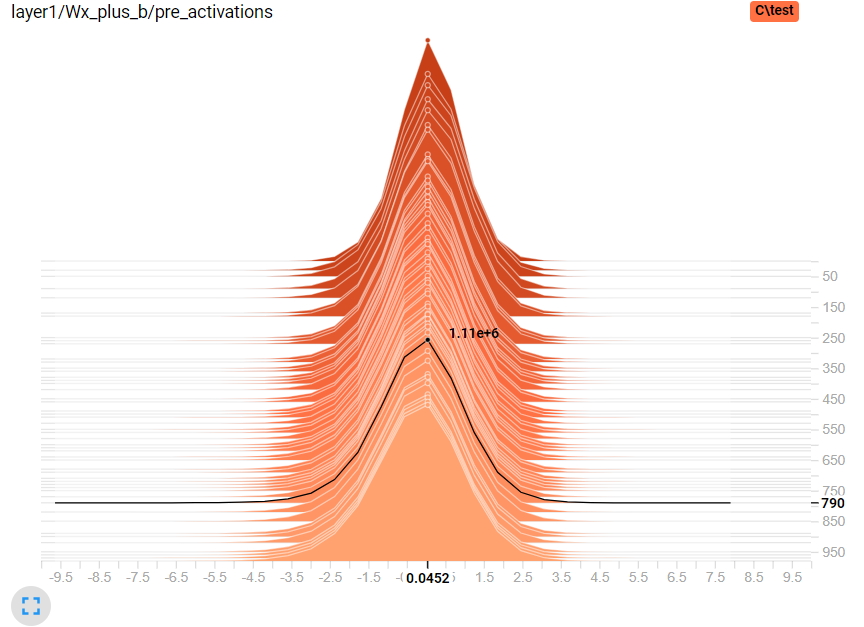
\includegraphics[width=0.7\textwidth]{images/Kapitel_3/histogram.png}\\
	\vspace{10pt} 
	\caption[Visualisierung eines Histogramms über die einzelnen Trainingsschritte]{Visualisierung eines Histogramms über die einzelnen Trainingschritte}
	\label{fig:histogram}
\end{figure}






\subsection{Verteilungen}
%\textbf{\textit{Verteilungen}}
\vspace{10pt}

Unter dem Reiter Verteilungen, welche ebenfalls mit der Klasse
\\

\begin{minipage}{\linewidth}
\begin{lstlisting} [label={lst:scalar}]
tf.summary.histogram(name, values, collections=None, familiy=None)
\end{lstlisting}
\end{minipage}
\vspace{0.2cm}

abgespeichert werden, befindet sich eine weitere Möglichkeit der Visualisierung der statistischen Verteilung. Hierbei repräsentiert die oberste Linie den über die Zeit veränderten maximalen Wert, die unterste Linie den minimalen Wert und die mittlere Linie den veränderten Median über der Zeit \cite{tensorboard.2017}.

\begin{figure}[h!]
	\centering
	%\vspace{-35pt}
	%\hspace{-1.0cm} 
	 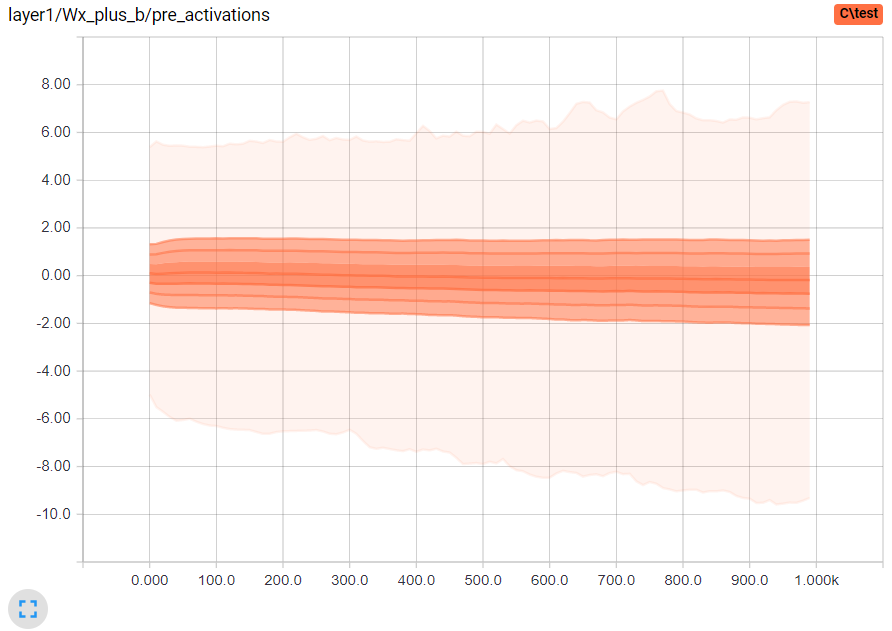
\includegraphics[width=0.6\textwidth]{images/Kapitel_3/distribution.png}\\
	\vspace{10pt} 
	\caption[Eine weitere Möglichkeit der Visualisierung der statistischen Verteilung]{Eine weitere Möglichkeit der Visualisierung der statistischen Verteilung}
	\label{fig:verteilung}
\end{figure}

%\vspace{0.3cm}



\subsection{Projektor}

%\textbf{\textit{Projektor}}

Die Auswahl des Reiters Projektors ermöglicht die höherdimensionale Visualisierung der Eingabedaten. Nachfolgend eine mögliche Konfiguration des Projektors:
\vspace{0.1cm}
\\

\begin{minipage}{\linewidth}
\begin{lstlisting} [label={lst:scalar}, caption={Konfiguration eines Projektors in TensorFlow \cite{embedding_viz}}]
from tensorflow.contrib.tensorboard.plugins import projector

# Use the same LOG_DIR where you stored your checkpoint.
summary_writer = tf.train.SummaryWriter(LOG_DIR)

# Format: tensorflow/contrib/tensorboard/plugins/projector/projector_config.proto
config = projector.ProjectorConfig()

# You can add multiple embeddings. Here we add only one.
embedding = config.embeddings.add()
embedding.tensor_name = embedding_var.name

# Link this tensor to its metadata file (e.g. labels).
embedding.metadata_path = os.path.join(LOG_DIR, 'metadata.tsv')

# Saves a configuration file that TensorBoard will read during startup.
projector.visualize_embeddings(summary_writer, config)
\end{lstlisting}
\end{minipage}
\vspace{0.3cm}

Hierbei werden zwei wesentliche Darstellungen unterschieden.
\vspace{10pt}

\begin{itemize} 
\item PCA (Prinicipal Component Analysis) \vspace{10pt}

Ein häufiges Problem bei multivariaten Daten ist, dass diese nicht im zweidimensionalem Raum dargestellt werden können.  Hierbei werden bei der Hauptkomponentenanalyse (PCA) die Daten so auf eine zweidimensionale (bzw. dreidimensionaler) Ebene projiziert, mit der Erwartung, dass diese neue Darstellung eventuell vorhandenes Rauschen herausfiltert und versteckte Strukturen zum Vorschein bringt \cite{pca}.
%http://www.statistics4u.info/fundstat_germ/cc_pca.html
\begin{figure}[h!]
	\centering
	%\vspace{-35pt}
	%\hspace{-1.0cm} 
	 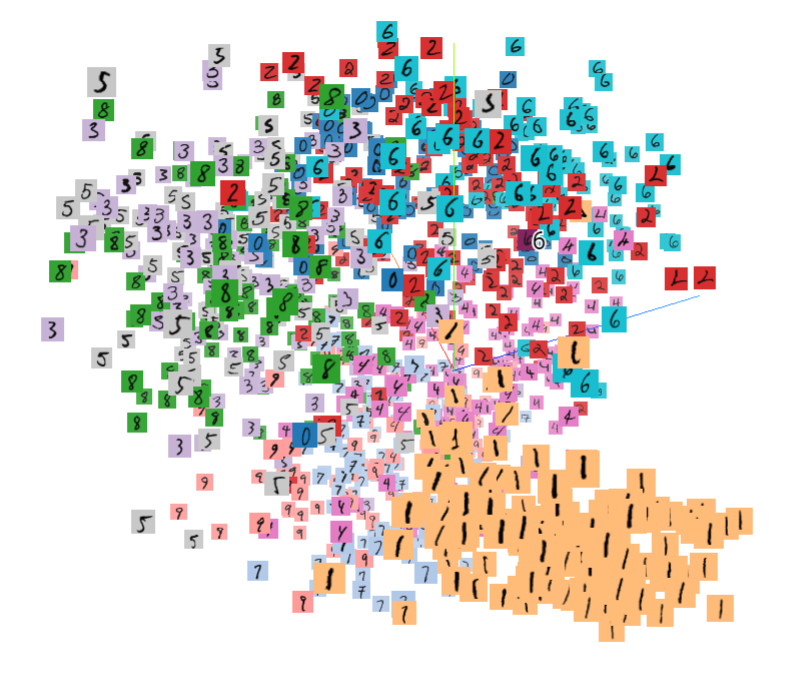
\includegraphics[width=0.6\textwidth]{images/Kapitel_3/projektor_pca.png}\\
	\vspace{10pt} 
	\caption[Visualisierung des PCA]{Visualisierung des PCA}
	\label{fig:pca}
\end{figure}



\item T-SNE (T-distributed Stochastic Neighbor Embedding) \vspace{10pt}

Diese Technik der Dimensionsreduktion eignet sich besonders gut, um hochdimensionale Daten in einen Raum von zwei oder drei Dimensionen zu projizieren. Hierbei wird jedes hochdimensionale Objekt durch einen zwei- oder dreidimensionalen Punkt modelliert, sodass ähnliche Objekte durch nahe gelegene Punkte und ungleiche Objekte durch entfernte Punkte modelliert werden \cite{t-sne}.


\begin{figure}[h!]
	\centering
	%\vspace{-35pt}
	%\hspace{-1.0cm} 
	 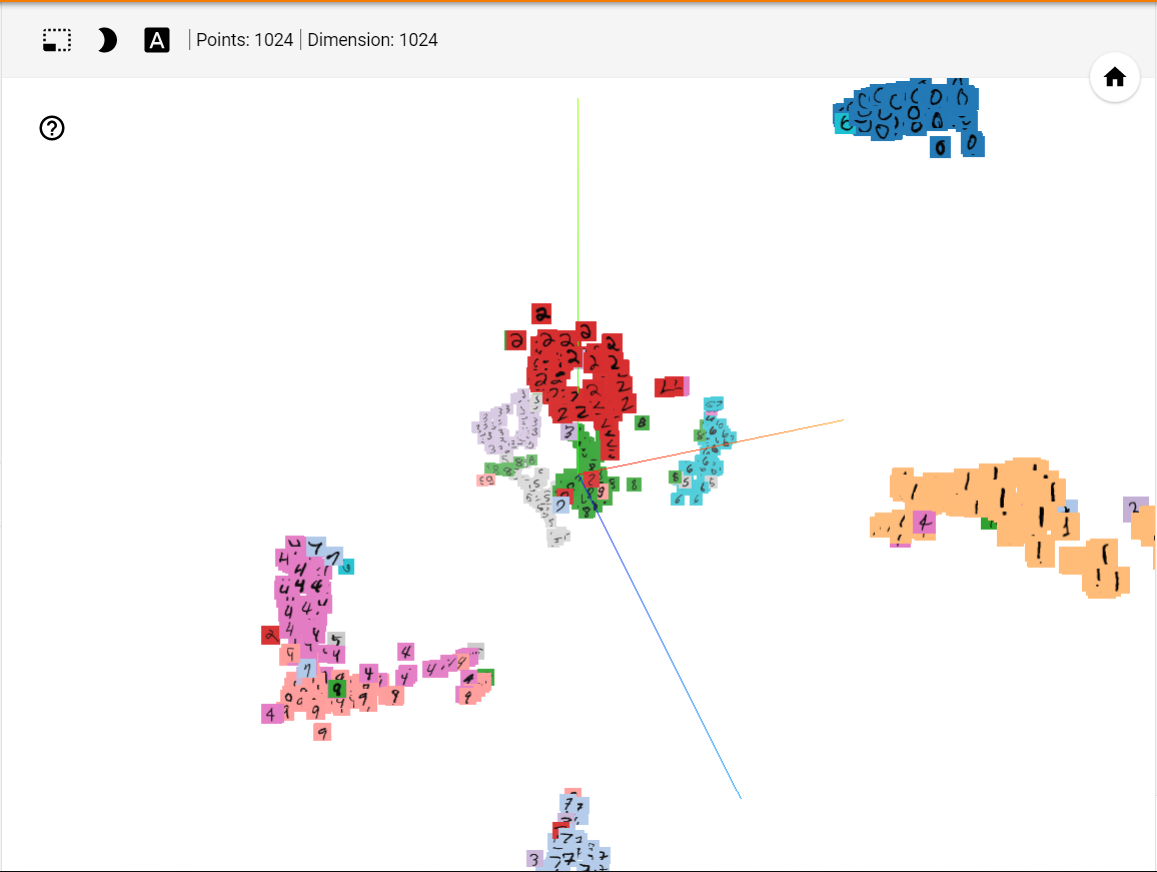
\includegraphics[width=0.6\textwidth]{images/Kapitel_3/projektor_t-sne.png}\\
	\vspace{10pt} 
	\caption[Visualisierung des T-SNE]{Visualisierung des T-SNE}
	\label{fig:t-sne}
\end{figure}

\end{itemize}


\subsection{Audio und Text}

Unter dem Reiter Audio können mit der Klasse
\\

\begin{minipage}{\linewidth}
\begin{lstlisting} [label={lst:scalar}]
tf.summary.audio(name, tensor, sample_rate, max_outputs=3, collections=None, family=None)
\end{lstlisting}
\end{minipage}
\vspace{0.2cm}

abspielbare Audio-Widgets eingebettet werden.\\

Ebenso können unter dem Reiter Text mit der Klasse
\\

\begin{minipage}{\linewidth}
\begin{lstlisting} [label={lst:scalar}]
tf.summary.text(name, tensor, collections=None)
\end{lstlisting}
\end{minipage}
\vspace{0.2cm}

Textausschnitte abgespeichert werden. Zusätzliche Funktionen wie Hyperlinks, Listen und Tabellen werden unterstützt \cite{tensorboard.2017}.





\newpage

\section{Die Graphelemente im Datenfluss}

 Dafür wurden zahlreiche unterschiedliche Elemente definiert, welche nachfolgend kurz erläutert werden \cite{graph_viz}.
\\

\begin{tabular}{ p{4cm}p{10.8cm} ll }

\textbf{Namespace} \tabularnewline 
\includegraphics[width=0.1\textwidth]{images/Kapitel_3/namespace.png}
\label{fig:namespace}
 & High-level Knoten repräsentiert einen definierten Namensbereich.   \tabularnewline
  
\textbf{Unconnected series} \tabularnewline 

\includegraphics[width=0.1\textwidth]{images/Kapitel_3/Unconnected_series.png}
\label{fig:Unconnected_series}
 & Nummerierte Knoten, die nicht miteinander verbunden sind. \tabularnewline
  
\textbf{Connected series} \tabularnewline 

\includegraphics[width=0.1\textwidth]{images/Kapitel_3/Connected_series.png}
\label{fig:Connected_series}
 & Nummerierte Knoten, die miteinander verbunden sind. \tabularnewline 
 
\textbf{Operation node} \tabularnewline 

\includegraphics[width=0.1\textwidth]{images/Kapitel_3/Operation_node.png}
\label{fig:Operation_node}
 & Ein Knoten der eine einzelne Operation darstellt.  \tabularnewline 
 
\textbf{Constant} \tabularnewline 

\includegraphics[width=0.08\textwidth]{images/Kapitel_3/Constant.png}
\label{fig:Constant}
 & Repräsentiert eine Konstante im Programm.  \tabularnewline 

\textbf{Summary node} \tabularnewline 

\includegraphics[width=0.07\textwidth]{images/Kapitel_3/Summary_node.png}
\label{fig:Summary_node}
 & Dieser Knoten stellt eine Zusammenfassung dar.  \tabularnewline 

\textbf{Dataflow edge} \tabularnewline 

\includegraphics[width=0.1\textwidth]{images/Kapitel_3/Dataflow_edge.png}
\label{fig:Dataflow_edge}
 & Durchgezogener Pfeil zeigt den Datenfluss zwischen den Operationen an.  \tabularnewline
 
\textbf{Control edge} \tabularnewline 

\includegraphics[width=0.1\textwidth]{images/Kapitel_3/Control_dependency_edge.png}
\label{fig:Control_dependendy_edge}
 & Gepunkteter Pfeil zeigt die Steuerungsabhängigkeit zwischen den Operationen an.  \tabularnewline 
 
\textbf{Reference edge} \tabularnewline 

\includegraphics[width=0.1\textwidth]{images/Kapitel_3/Reference_edge.png}
\label{fig:Reference_edge}
 & Gelber Pfeil bedeutet, dass die ausgehende Operation die ankommende mutieren kann   \tabularnewline 
% & \tabularnewline
\end{tabular}
\\
